\documentclass[12 pt, a4paper]{article}
\usepackage[utf8]{inputenc}
\usepackage[left=2.5 cm,top=2.54 cm,right=2.5 cm,bottom=2.54 cm]{geometry}
\usepackage[flushleft]{threeparttable}
\usepackage{mathtools}
\usepackage{amssymb}
\usepackage{amsmath}
\title{Linear Statistical Models Assignment 1} 
\date{}
\usepackage[dvipsnames]{xcolor}
\usepackage{graphicx,wrapfig}
\author{Kim Seang CHY}
\usepackage{xcolor}

%Table Adjustment
\usepackage{tabularx}
\newcommand{\tabitem}{~~\llap{\textbullet}~~}

\begin{document}

\maketitle


\section*{Question 1}
\textbf{a.} For a symmetric matrix \textbf{A}, if $\textbf{A}^2=\textbf{A}^3$, then \textbf{A} is idempotent.\\

\noindent There are two cases the first is the first is matrix \textbf{A} over $\mathbb{R}$ and the second case is matrix \textbf{A} over $\mathbb{C}$.\\

\noindent \textbf{Case 1:} Let \textbf{A} be a symmetric matrix over $\mathbb{R}$ such that $\textbf{A}^2=\textbf{A}^3$.\\

\noindent By eigenvalue properties,  \textbf{A} is diagonalisable with real eigenvalues and orthogonal eigenvectors, thus there exist a diagonalise matrix \textbf{P} such that:
\begin{align*}
\textbf{P}^T\textbf{AP}=\textbf{D}
\end{align*}
where \textbf{D}=diag$(\lambda_1,\lambda_2, \ldots,\lambda_i,\ldots)$ and $\lambda_i$ is the eigenvalue of A for all $i \in \mathbb{N} \setminus \{0\}$ \\

\noindent Since $\textbf{A}^2=\textbf{A}^3$,  this implied:
\begin{align*}
&\textbf{D}^2=\textbf{D}^3 &\text{(Diagonalise relationship)} \\
&\implies (\lambda_i)^2=(\lambda_i)^3,  \hspace{0.15cm} \forall i \in \mathbb{N} \setminus \{0\} &\\
&\implies \lambda_i^2(\lambda_i-1) = 0  & \\
&\implies \lambda_i =0 \text{ or } \lambda_i = 1 \\
\end{align*}

\noindent Since the eigenvalue can only take value of 0 or 1.  We can inferred:
\begin{align*}
&\textbf{D}=\textbf{D}^n,  \hspace{0.1cm} n=1,2,3\ldots & (\text{Diagonal matrix properties })\\
&\implies \textbf{A}=\textbf{A}^n & (\text{By diagonalisaiton properties})
\end{align*}



Given $\textbf{A}=\textbf{A}^{n}$. Hence,\textbf{A} is an idempotent matrix by the definition of idempotent matrix and its diagonalise properties.  The statement is true if \textbf{A} is a real matrix and symmetric.\\

\noindent \textbf{Case 2}: Proof by counter example. \\

\noindent Let \[ \textbf{A} = 
\begin{bmatrix}
- \textbf{i} & 1 \\
1 & \textbf{i} \\
\end{bmatrix}
\]
Notice that $\textbf{A} = \textbf{A}^T$, this implied \textbf{A} is a symmetric matrix.  Now notice that:
\[ \textbf{A}^2 = 
\begin{bmatrix}
0 & 0 \\
0 & 0 \\
\end{bmatrix}
= \textbf{0}
\]
This implied $\textbf{A}^3=\textbf{0A}=\textbf{0}=\textbf{A}^2$. However,  $\textbf{A} \neq \textbf{A}^2$, thus \textbf{A} is not idempotent.  Hence, the statement is false for a complex symmetric matrix. 

Therefore,   a symmetric matrix \textbf{A} such that $\textbf{A}^2=\textbf{A}^3$, implied \textbf{A} is idempotent if and only if \textbf{A} has all real element. \\


\noindent \textbf{b.} For a symmetric matrix \textbf{A}, if $\textbf{A}=\textbf{A}^3$, then \textbf{A} is idempotent.\\

\noindent \textbf{Proof:} Proof by counter example.
 \[ \text{Let }\textbf{A} =
\begin{bmatrix}
1 & 0 \\
0 & -1
\end{bmatrix}
\]
Notice that \textbf{A} = $\textbf{A}^T$,  this implied \textbf{A} is a symmetric by definition of symmetric.  \\
\[ \textbf{A}^2 = 
\begin{bmatrix}
1 & 0 \\
0 & 1 \\
\end{bmatrix}
\]
\[
\textbf{A}^3 = \begin{bmatrix}
1 & 0 \\
0 & -1 \\
\end{bmatrix}
\] 
$\textbf{A} \neq \textbf{A}^2$,  hence \textbf{A} is not idempotent.  Since $\textbf{A}=\textbf{A}^3$ but \textbf{A} is not idempotent. Therefore,  the statement is false.  

\section*{Question 2:} 

Prove for $A_1,A_2, \ldots,  A_m$ set of symmetric $k \times k$ matrices and there exist an orthogonal matrix \textit{P} such that $P^TA_iP$ is diagonal for all $i$ then $A_iA_j=A_jA_i$ for every pair of $i,j = 1,2,\ldots, m$.\\


\noindent \textbf{Proof:}\\
Supposed $A_1$ and $A_2$ are symmetric $k \times k$ matrices,  simultaneously diagonalisable by orthogonal matrix $P$.  This implied there exist:
\begin{align*}
A_1= PD_1P^T
\end{align*}
and
\begin{align*}
A_2 = PD_2P^T
\end{align*}
Where $D_1$ is the diagonal matrix contain its respective eigenvalue for $A_1$ and  $D_2$ is the diagonal matrix contain its respective eigenvalue for $A_2$ \\

\noindent Hence:
\begin{align*}
A_1A_2 &=  PD_1P^TPD_2P^T \\
 & = PD_1D_2P^T & (P^TP = I \text{ by othrogal matrix properties})
\end{align*}
Since diagonal matrix are commutable this implied $D_1D_2=D_2D_1$. Therefore: \\
\begin{align*}
A_1A_2 &= PD_2D_1P^T \\
&= PD_2P^TPD_1P=A_2A_1
\end{align*}

The above can expand to be show for any set of symmetric matrix that is simultaneously diagonalisable by the same orthogonal matrix.  Therefore, if a set of symmetric matrices $A_1,A_2, \ldots,  A_m$ is simultaneously diagonalisable by $P$ then $A_iA_j=A_jA_i$ for every pair of $i,j = 1,2,\ldots, m$.

\section*{Question 3:}
Let \textbf{A} be an $n \times p$ matrix with rank p and all element belong to $\mathbb{R}$. This implied column vector of \textbf{A} is linearly independent.   Let \textbf{y} be a $p \times 1$ matrix such that \textbf{y} = $[y_1,y_2, \ldots,y_p]^T$. \\

\noindent Note that: 
\begin{align*}
\textbf{y}^T\textbf{A}^T \textbf{Ay} =( \textbf{Ay})^T \textbf{Ay} & &\text{(By the symmetric properties)}
\end{align*}
For \textbf{Ay} matrix, it can be represented in a from $\textbf{Ay}=\textbf{a}_1y_1+\textbf{a}_2 y_2+\ldots+\textbf{a}_py_p$ where $\textbf{a}_i$ represent the column vectors for matrix \textbf{A} for column \textit{i} where $i = 1,2,\ldots, p$. \\

\noindent Since the column are linearly independent, this implied there a non-zero solution to \textbf{Ay}=0 expect for $\textbf{y}=\textbf{0}$, thus implied there are also non-zero solution to$\textbf{y}^T\textbf{A}^T \textbf{Ay}$=0. Since $\textbf{y}^T\textbf{A}^T \textbf{Ay}=(\textbf{a}_1y_1)^2+(\textbf{a}_2 y_2)^2+\ldots+(\textbf{a}_py_p)^2$ , this this is just a sum of squares,  which implied $\textbf{y}^T\textbf{A}^T \textbf{Ay} > 0$ for all $y \in \mathbb{R} \setminus \{0\}$. Therefore,  $\textbf{y}^T\textbf{A}^T \textbf{Ay}$ is positively defined matrix.

\section*{Question 4:}
\textbf{a.} Let \textbf{y}=\textit{A}\textbf{x}. Find \textbf{A}.\\

\noindent Want to find a vector A such that: $\textbf{y}=A\textbf{x}=\textbf{x}-\textbf{1}\bar{x} $ where \textbf{1} is a column vector of 1 with three rows. \\
Notice that:
\begin{align*}
\bar{x}&=\frac{1}{3}\textbf{1}^T\textbf{x} \\
\implies \textbf{x}-\bar{x}\textbf{1}&= \textbf{x}-\frac{1}{3}\textbf{1}\textbf{1}^T\textbf{x} \\
 &=(\textbf{I}-\frac{1}{3}\textbf{11}^T)\textbf{x}\\
 \implies A &= \textbf{I}-\frac{1}{3}\textbf{11}^T
\end{align*}
\[
 \textbf{I}-\frac{1}{3}\textbf{11}^T = 
 \begin{bmatrix}
 1 & 0 & 0 \\ 
 0 & 1 & 0 \\
 0 & 0 & 1\\
 \end{bmatrix} - \frac{1}{3}
 \begin{bmatrix}
1 \\ 1 \\ 1
 \end{bmatrix}
  \begin{bmatrix}
1 \\ 1 \\ 1
 \end{bmatrix}^T = 
 \begin{bmatrix}
 \frac{2}{3} & \frac{-1}{3} & \frac{-1}{3} \\
 \frac{-1}{3} & \frac{2}{3} & \frac{-1}{3} \\
 \frac{-1}{3} & \frac{-1}{3} & \frac{2}{3} \\
 \end{bmatrix}
\]
Hence \[ A = \begin{bmatrix}
\frac{2}{3} & \frac{-1}{3} & \frac{-1}{3} \\
 \frac{-1}{3} & \frac{2}{3} & \frac{-1}{3} \\
 \frac{-1}{3} & \frac{-1}{3} & \frac{2}{3} \\
\end{bmatrix}
\]

\noindent \textbf{b.} Find the rank of A.\\

\noindent The rank(A) = 2, since the sum of column 1 and column 2 is equal to negative of column 3 and column 1 is not a multiple of column 2. 


\noindent \textbf{c.} Find E($\textbf{y}^T\textbf{y}$).


\[\text{E}(\textbf{y}^T\textbf{y}) = E \left(
\begin{bmatrix}
x_1-\bar{x} \\ x_2-\bar{x} \\ x_3-\bar{x}
\end{bmatrix}^T
\begin{bmatrix}
x_1-\bar{x} \\ x_2-\bar{x} \\ x_3-\bar{x}
\end{bmatrix} \right)
\]

\begin{align*}
=\text{E}\left(\sum_{i=1}^3(x_i-\bar{x})^2\right) \\
=\text{E}\left[\sum_{i=1}^3x_i \right]-\text{E}\left[3\bar{x}^2\right]\\
=\sum_{i=1}^3E[x_i^2]-3\text{E}[\bar{x}^2]
\end{align*}
Notice that Var($x$)=E($x^2)-(\text{E}(x))^2$,  this implied E($x^2) = \text{Var}(x)+(\text{E}(x))^2 = \sigma^2+\mu^2$. \\
Similarly, Var($\bar{x}$)=E($\bar{x}^2)-(\text{E}(\bar{x}))^2$, this implied E($\bar{x}^2)= \text{Var}(\bar{x})+\text{E}(\bar{x}) ^2=\frac{\sigma^2}{3}+\mu^2$, since $x_1,x_2,x_3$ is IID Therefore, 

\begin{align*}
\text{E}(\textbf{y}^T\textbf{y}) &=\left[ \sum_{i=1}^3(\sigma^2+\mu^2) - 3\left(\frac{\sigma^2}{3}+\mu^2 \right)\right]\\
& = \left[(\sigma^2+\mu^2)-3\left(\frac{\sigma^2}{3}+\mu^2 \right)\right]= \left[2\sigma^2 \right]
\end{align*}

\noindent \textbf{d.} Using theorem 3.5, find the distribution of $\frac{\textbf{y}^T\textbf{y}}{\sigma^2}$. \\

\noindent From part 1 we know $\textbf{y}=A\textbf{x}$ and $\textbf{x}\sim MVN(\mu,\sigma^2)$ is $3 \times 1$ random vectors and
\begin{align*}
\text{A}& =
\begin{bmatrix}
\frac{2}{3} & \frac{-1}{3} & \frac{-1}{3} \\
 \frac{-1}{3} & \frac{2}{3} & \frac{-1}{3} \\
 \frac{-1}{3} & \frac{-1}{3} & \frac{2}{3} \\
\end{bmatrix} \\
\implies A^2&=
\begin{bmatrix}
\frac{2}{3} & \frac{-1}{3} & \frac{-1}{3} \\
 \frac{-1}{3} & \frac{2}{3} & \frac{-1}{3} \\
 \frac{-1}{3} & \frac{-1}{3} & \frac{2}{3} \\
\end{bmatrix}
\end{align*}

Notice that $A=A^T$ and $A=A^2$, this implies $A$ is a symmetric and idempotent  matrix.  Thus: \\

\begin{align*}
\frac{\textbf{y}^T\textbf{y}}{\sigma^2}&=\frac{1}{\sigma^2}(A\textbf{x})^T(A\textbf{x}) \\
&=\frac{1}{\sigma^2}\textbf{x}^TA^TA\textbf{x} \\
&=\frac{1}{\sigma^2}\textbf{x}^TA^2\textbf{x} \\
&=\frac{\textbf{x}}{\sigma}^TA\frac{\textbf{x}}{\sigma}
\end{align*}

\noindent Since $\sigma$ is a constant this implied $\frac{1}{\sigma}\textbf{x} \sim MVN(\frac{1}{\sigma}\mu, \sigma^2)$.  Therefore, by Theorem 3.5,  implied $\frac{\textbf{y}^T\textbf{y}}{\sigma^2}$ has a noncentral $\chi^2$ with rank($A)=2$ degree of freedoms, and a noncentral parameter $\lambda=\frac{1}{2}\left(\frac{\boldsymbol{\mu}}{\sigma}\right)^TA\left(\frac{\boldsymbol{\mu}}{\sigma}\right)=\frac{1}{2\sigma^2}\boldsymbol{\mu}^TA\boldsymbol{\mu}$. In this case: \[ \lambda = \frac{1}{2\sigma^2} 
\begin{bmatrix}
\mu \\ \mu \\ \mu
\end{bmatrix} ^T
\begin{bmatrix}
\frac{2}{3} & \frac{-1}{3} & \frac{-1}{3} \\
 \frac{-1}{3} & \frac{2}{3} & \frac{-1}{3} \\
 \frac{-1}{3} & \frac{-1}{3} & \frac{2}{3} \\
\end{bmatrix}
\begin{bmatrix}
\mu \\ \mu \\ \mu
\end{bmatrix}
=[0]
\]
Since $\lambda=0$,  this implied $\frac{\textbf{y}^T\textbf{y}}{\sigma^2}$ is regular $\chi^2$ distribution with 2 degree of freedom.


\section*{Question 5:}

\noindent All the matrix calculation and other calculation for this question will be in appendix.\\

\noindent \textbf{a.} Write down the matrices and vector involved in the linear model $\textbf{y}=\textbf{X} \boldsymbol{\beta}+ \boldsymbol{\epsilon}$. \\

\noindent Since,  we are trying to model the price of fish in 1980,  based on the 1970 price then the predictor variables($y_i$) is the price of fish in 1980 and the explanation variable $x_{i2}$ is the price of fish in 1970.  The model $\textbf{y}=\textbf{X} \boldsymbol{\beta}+ \boldsymbol{\varepsilon}$ is given by:

\[
\begin{bmatrix}
27.3 \\ 42.4 \\ 38.7 \\ 4.5 \\ 23 \\ 166.3 \\ 109.7 \\ 80.1 \\ 150.7 \\ 20.3 \\ 189.7 \\ 131.3 \\404.2 \\149
\end{bmatrix}=
\begin{bmatrix}
1 & 13.1 \\ 1 & 15.3 \\ 1 & 25.8 \\ 1 & 1.8 \\ 1 & 4.9 \\ 1 & 55.4 \\ 1 & 39.3 \\ 1 & 26.7\\ 1 &  47.5 \\ 1 & 6.6 \\ 1 & 94.7 \\ 1 & 61.1 \\ 1 & 135.6\\ 1 & 47.6
\end{bmatrix}
\begin{bmatrix}
\beta_0 \\ \beta_1
\end{bmatrix} + 
\begin{bmatrix}
\varepsilon_1 \\ \varepsilon_2 \\ \vdots \\ \varepsilon_{14}
\end{bmatrix}
\]
Where $\beta_0, beta_1$ are the parameter and $\varepsilon_i$ are the error term in row i. \\


\noindent \textbf{b.} Find the least squares estimators of the parameters.

\[ \text{Let \textbf{b}} = 
\begin{bmatrix}
b_0 \\ b_1 
\end{bmatrix}
\]

\noindent By theorem 4.4, the best least estimator is give by: $\textbf{b}= (X^TX)^{-1}X^T\textbf{y}$. 

\begin{align*}
X^TX& = 
\begin{bmatrix}
14.0 & 575.4 \\
575.4 & 42079.36\\
\end{bmatrix} \text{ and } (X^TX)^{-1} = 
\begin{bmatrix}
0.16308 & -0.0022 \\
-0.0022 & 5.43\text{e-5}
\end{bmatrix} 
\end{align*}

\begin{align*}
\implies \textbf{b} &= (X^TX)^{-1}X^T\textbf{y} \\
&= \begin{bmatrix}
-1.2338 \\ 2.7016
\end{bmatrix}
\end{align*}

\noindent The least square estimator $b_{0}=-1.2338$ with var$(b_{0}) = 0.163 \sigma^{2}$ and $b_1=2.7016$ with var$(b_{1})=(5.43 \text{e-5})  \sigma^2$.\\


\noindent \textbf{c.} Find the sample variances $s^2$. \\

\noindent By theorem 4.6,  the unbiased for $\sigma^2$ is given by:
\begin{align*}
s^2=\frac{(\textbf{y}-X\textbf{b})^T(\textbf{y}-X\textbf{b})}{n-(k+1)}
\end{align*}

\noindent Where n is row of \textbf{x} and \textbf{y} and $k+1$ is the column of \textbf{x}. Hence for our data sets
\begin{align*}
s^2&= \frac{(\textbf{y}-X\textbf{b})^T(\textbf{y}-X\textbf{b})}{14-2}\\
& = \frac{9325.833}{12} = 777.1528
\end{align*}
The sample variance for our model is 777.1528.  \\

\noindent Since the variance of the parameter is given by var(\textbf{b}) $=(X^TX)^{-1}\sigma^2$ or $(X^TX)^{-1}s^2$,  this implied var($b_0)=126.74$ and var($b_1)=0.04217$\\

\noindent \textbf{d. } Predict the price for ocean trout in 1980 given a fisher sold ocean trout for 28c/pound in 1970.

\[ \text{Let } t= 
\begin{bmatrix}
1 \\ 28
\end{bmatrix}
\]

\noindent By theorem 4.5,  we can uses $\textbf{t}^T\textbf{b}$ we can use to predict the price as it is best linear unbiased estimator for $\textbf{t}^T\boldsymbol{\beta}$.\\
Therefore,  to predict the  of ocean trout given fisher sold ocean trout for 28c/pound and our model:
\begin{align*}
\text{price}_{1980} &= -1.2338+2.7016\text{ price}_{1970} \\
&= \begin{bmatrix}
1 \\ 28
\end{bmatrix}^T 
\begin{bmatrix}
-1.2338 \\ 2.7016
\end{bmatrix}
= [74.40965]
\end{align*}

The price for ocean trout the fisherman expected get in 1980 is \$74.41c /pound.   \\

\noindent \textbf{e.} Calculate the standardised residual for sea scallops.\\

\noindent Let $H=X(X^TX)^{-1}X^T$ and $\textbf{e}=\textbf{y}-X\textbf{b}$.  Hence $H_{13 \text{ }  13}=0.5560$ and $\textbf{e}_{13 \text{ }  1}=39.10$ since the sea scallop is in the 13th index of our data \\

\noindent The standardised residual is given by: \\
\begin{align*}
z_i&=\frac{e_{1i}}{\sqrt{s^2(1-H_{ii}})} \\
\implies z_{13}&=\frac{39.10}{\sqrt{777.1528(1-0.5560)}}=2.104999
\end{align*}

\noindent The standardised residual for sea scallops is 2.1050. \\

\noindent \textbf{f.} Calculate the Cook’s distance for sea scallops.\\

\noindent The Cook's distance for sea scallops is:

\begin{align*}
D_{13}&=\frac{z_{13}^2}{1+1} \left( \frac{H_{13 \text{ } 13}}{1-H_{13 \text{ } 13}} \right) \\
& = \frac{2.1050^2}{2} \left(  \frac{0.5560}{1- 0.5560} \right) =2.7740
\end{align*}

\noindent \textbf{g.} Does sea scallops fit the linear model? Justify your argument.\\

\noindent The sea scallops Cook's distance is 2.774 which is significantly greater than 1 thus implied the sea scallops observation is a point of high leverage and high standardised residual.  Such point is considered to be an influential outlier that significant impact the fit a model hence the sea scallops does not fit the linear model.  \\

\noindent This was also reflected in best fit line of the graph below where the best fit line without sea scallops observation is steeper than the best fit line with sea scallops observation.

\begin{figure}[h]
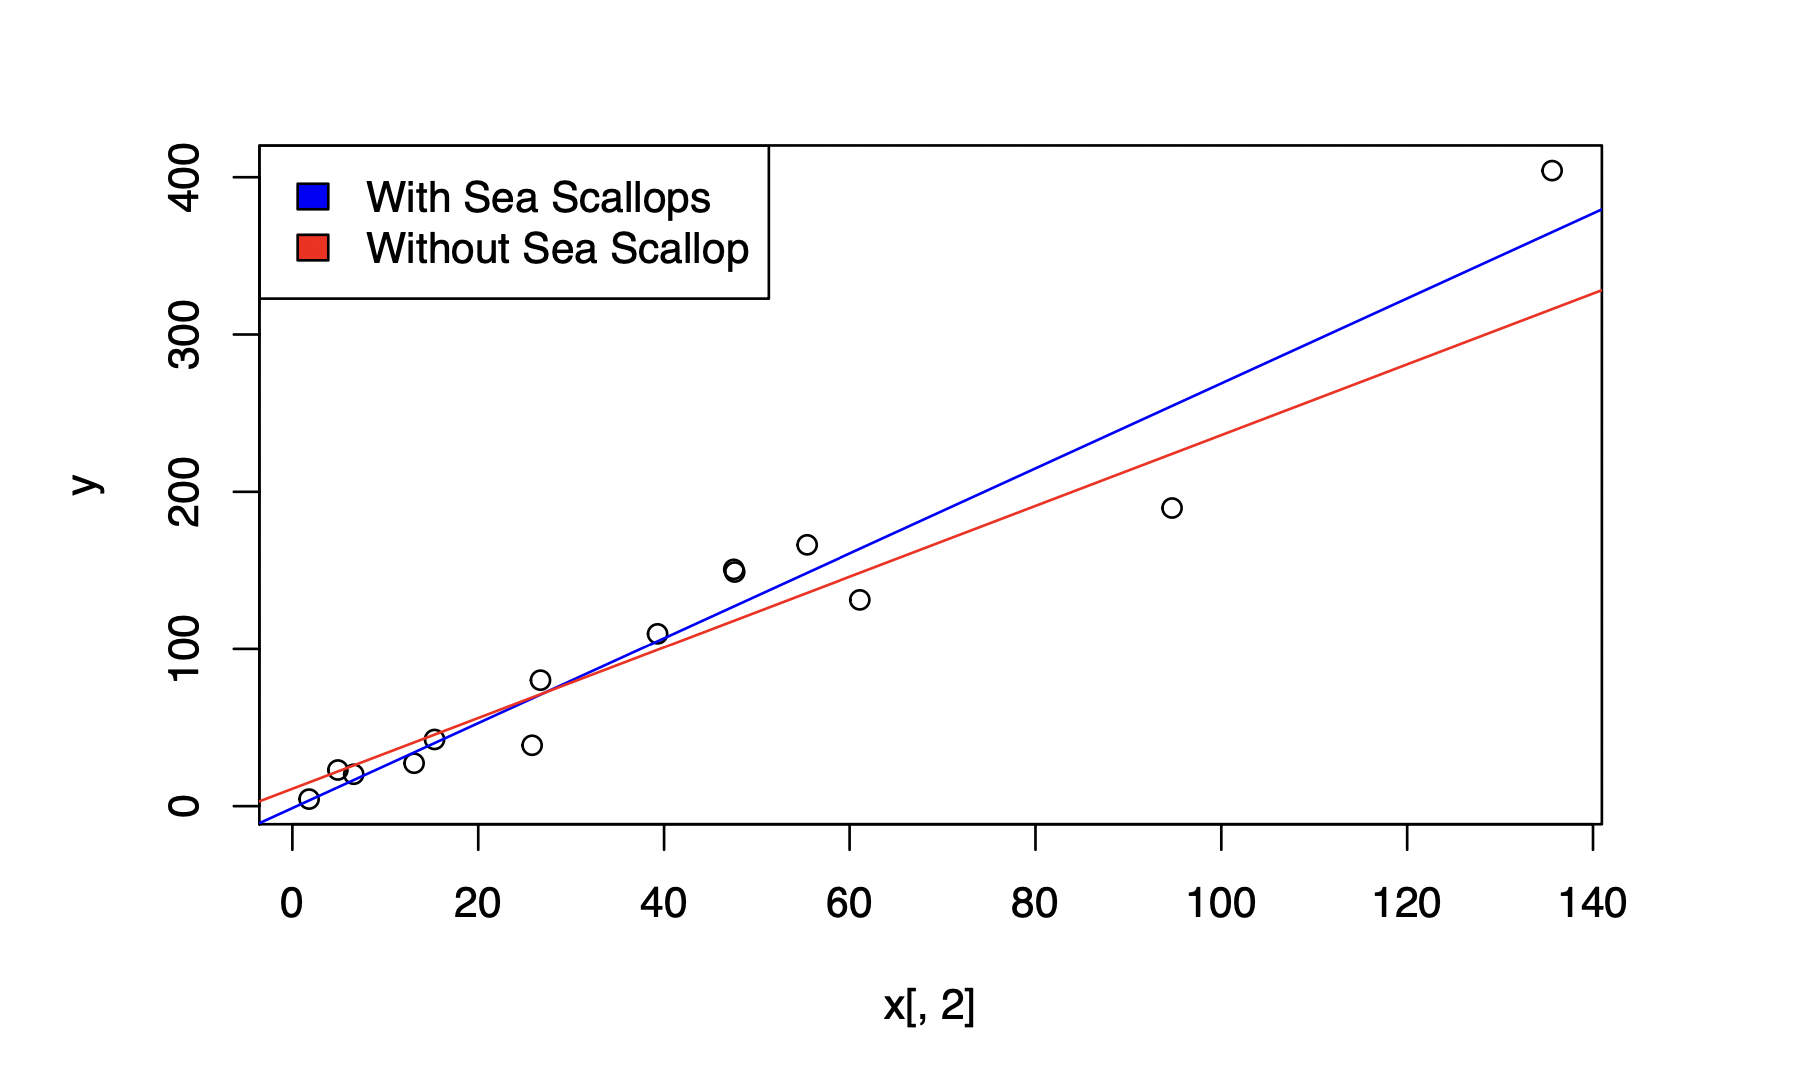
\includegraphics[scale =0.3]{graph00}
\end{figure}

















\end{document}